
\documentclass[]{article}
\usepackage{framed}
\usepackage{amsmath}
\usepackage{amssymb}
\usepackage{multicol}
\usepackage{graphicx}
%opening

\begin{document}

%---------------------------------------%
\section*{Question 3 (Sample Variant 2)[25 marks]}
\begin{itemize}
%--------------------------------- %
\item[(a)] \textbf{\textit{Normal Probability Distribution (8 Marks)}}\\
A well known IT retailer has determined that the number of computer accessories sold, on a weekly basis in its largest shop, is normally distributed with a mean of 1200 and standard deviation of 50.
\begin{itemize}
\item[(i)] (2 Marks) Estimate the proportion of weeks that the company will sell more than 1175 products.

\item[(ii)] (3 Marks) Estimate the proportion of weeks that the company will sell less more than 1150 products.
\item[(iii)] (3 Marks) Estimate the proportion of weeks that the company will sell between 1175
products and 1275 products?
\end{itemize}
%--------------------------------- %

\item[(b)] \textbf{\textit{Theory of Statistical Inference (6 Marks)}}\\Answer the following questions on the theory of statistical inference.
\begin{itemize}
\item[(i)] (2 Marks) What is a $p-$value?
\item[(ii)] (2 Marks) Briefly describe how $p-$value is used in hypothesis testing.
\item[(iii)] (1 Mark) What is meant by a Type I error?
\item[(iv)] (1 Mark) What is meant by a Type II error?
\end{itemize}
%--------------------------------- %
\bigskip

\item[(c)] \textbf{\textit{Confidence Intervals (4 Marks)}}\\
A press release for a broadband provider stated that $90\%$ percent of customers are very satisfied
with the standard of service. To test this claim, the local chamber of commerce surveyed 210 randomly selected customers. Among the sampled customers, 182 stated that they are very satisfied.


%Test the hypothesis that $90\%$ of all customers are very satisfied with their service. You may assume a significance level of 5\%.



\begin{itemize}
\item[(i)] (1 Mark) Compute the appropriate value for the standard error for a confidence interval.
\item[(ii)] (2 Marks) Compute the 95\% confidence interval for $\pi$, the true proportion.
%\item[iii] (2 marks) For the test statistic, determine the corresponding p-value.
\item[(iii)] (1 Mark) What is your conclusion for this claim made by the press release? Justify your answer.
\end{itemize}
%--------------------------------- %
\end{itemize}

%
\newpage
\begin{itemize}
%---------------------------------- %
\item[(d)] \textbf{\textit{ Inference Procedures with \texttt{R} (6 Marks)}}\\
Consider the following inference procedure performed on data set $X$.
\begin{center}
\begin{framed}
\begin{verbatim}
> var.test(X,Z)

        F test to compare two variances

data:  X and Z 
F =........, num df = 13, denom df = 11, p-value = 0.7813
alternative hypothesis: 
   true ratio of variances is not equal to 1 
95 percent confidence interval:
 0.2526643 2.7401535 
sample estimates:
ratio of variances 
         ........

\end{verbatim}
\end{framed}
\end{center}
\textit{(MA4413 2013 - will not be asked to compute the Test Statistic)}
\begin{itemize}
\item[(i)] (1 Mark) Describe what is the purpose of this statistical procedure.
\item[(ii)] (2 Marks) What are the null and alternative hypotheses?
\item[(iii)] (1 Mark) Write the conclusion that follows from the code output, displayed above.
\end{itemize}
\end{itemize}

%---------------------------------- %
\begin{itemize}
\item[(e)] \textbf{\textit{Graphical Procedures (3 Marks)}}
\begin{itemize}
\item[(i)] (2 Marks) The graph below depicts a normal probability plot. Describe what this plot is used for and how to interpret one.
\item[(ii)](1 Mark) What is your conclusion for the data used to construct the normal probability plot below.
\end{itemize}
\begin{center}
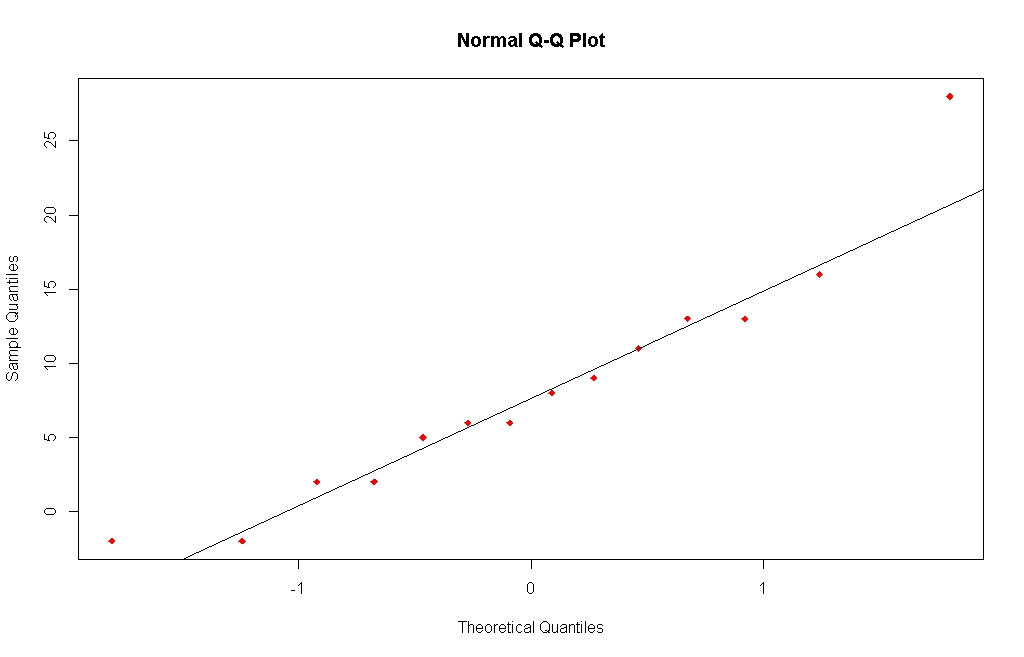
\includegraphics[scale=0.38]{10AQQplot}
\end{center}
\end{itemize}
\end{document}